\section{Experimental Evaluation}
\label{sec:exp}

We conduct experiments to answer five main questions: (1) can \methodname\ prevent degradation in performance when sharing data as observed in Section~\ref{sec:analysis}?, (2) how does \methodname\ compare to vanilla multi-task offline RL methods and prior data sharing methods?,
(3) can \methodname\ handle sparse reward settings where data sharing is particularly important due to scarce supervision signal?, (4) can \methodname\ handle goal-conditioned offline RL settings where the offline dataset is undirected and highly suboptimal?, and (5) Is \methodname\ able to scale to raw visual observations?

\textbf{Comparisons.} To answer these questions, we consider the following prior methods. On tasks with low-dimensional state spaces, we compare with the online multi-task relabeling approach \textbf{HIPI}~\citep{eysenbach2020rewriting}, which uses inverse RL to infer for which tasks the datapoints are optimal and in practice routes a transition to task with the highest Q-value. We adapt HIPI to the offline setting by applying its data routing strategy to a conservative offline RL algorithm.
We also compare to na\"ively sharing data across all tasks (denoted as \textbf{Sharing All}) and vanilla multi-task offline RL method without any data sharing (denoted as \textbf{No Sharing}). On image-based domains, we compare \methodname\ to the data sharing strategy based on human-defined skills~\citep{kalashnikov2021mt} (denoted as \textbf{Skill}), which manually groups tasks into different skills (e.g. skill ``pick'' and skill ``place'') and only routes an episode to target tasks that belongs to the same skill of the source task.
Similar to the low-dimensional settings, we also compare to \textbf{HIPI}, \textbf{Sharing All} and \textbf{No Sharing}. We use CQL~\citep{kumar2020conservative} as the base offline RL algorithm for all methods. For more details on the experiment set-up and hyperparameters, see Appendix~\ref{app:details}.


\textbf{Multi-task locomotion domains.} To answer question (1) and (2), we consider three locomotion environments from OpenAI Gym~\citep{brockman2016openai} with dense rewards: halfcheetah, walker2d, and ant. We show results of walker2d here and leave the results of halfcheetah and ant to Appendix~\ref{app:additional_exp}. We follow the set-up discussed in Section~\ref{sec:analysis}. Specifically, we create three tasks, \texttt{run forward}, \texttt{run backward} and \texttt{jump}, which are used in prior offline RL works~\citep{yu2020mopo}. We visualize the environment in Figure~\ref{fig:env}. As shown in Section~\ref{sec:analysis} and Table~\ref{tab:analysis}, data sharing would lead to performance degradation in settings where we have large diverse datasets (medium-replay) for \texttt{run forward}, medium-sized datasets (medium) for \texttt{run backward} and expert datasets with limited data (expert) for \texttt{run jump}, we evaluate \methodname\ on exactly this setting to see \methodname\ can prevent harmful data sharing and instead exploit the shared structure among tasks and help training.

\begin{table*}[t!]
\centering
\vspace*{0.1cm}
\scriptsize
\begin{tabular}{l|l|r|r|r|r}
\toprule
\textbf{Environment} & \textbf{Tasks / Dataset type} & \textbf{\methodname\ (ours)}& \textbf{HIPI}~\cite{eysenbach2020rewriting}& \textbf{Sharing All} & \textbf{No Sharing}\\ \midrule
% & run forward / medium-replay & 2587.7  & \textbf{2626.1} & 2605.0 & \textbf{2632.5}\\
% halfcheetah & run backward / medium & 2519.5  & \textbf{2634.4} & \textbf{2636.7} & \textbf{2630.7}\\
% & jump / expert & \textbf{4298.2} & 4113.4 & 712.3 & -1978.3\\
% & \CC \textbf{average} & \CC \textbf{3135.1} & \CC \textbf{3124.7} & \CC 1984.7 & \CC 1095.0\\
% \midrule
& run forward / medium-replay & \textbf{1100.7} & 692.2 & 701.4 & 590.1\\
walker2d & run backward / medium & 638.4 & 664.9& \textbf{756.7}& 614.7\\
& jump / expert & 1538.4  & \textbf{1604.4} & 885.1 & 1575.2\\
& \CC \textbf{average} & \CC \textbf{1092.5} & \CC 987.2 & \CC 781 & \CC 926.6\\\midrule
% & run forward / medium-replay & 2350.1 & \textbf{2658.9} & 1175.0 & 2126.7\\
% ant & run backward / medium & 1435.7 & 1208.2 & 1488.7 & \textbf{2021.7}\\
% & jump / expert & \textbf{2781.3} & 2670.4 & 133.8 & 495.8\\
% & \CC \textbf{average} & \CC \textbf{2189.0} & \CC \textbf{2179.2} & \CC 932.5 & \CC 1548.1\\
% \midrule
& door open / medium-replay & \textbf{57.3\%} & 30.7\% & 19.1\% & 0\%\\
& door close / expert & \textbf{33.3\%} & 0\% & 21\% & 2\% \\
Meta-World~\citep{yu2020metaworld}& drawer open / expert & 76\%  & 45.3\% & \textbf{85.5\%} & 0\%\\
& drawer close / medium-replay & 99.7\% & 66.7\% & \textbf{100\%} & 5.7\%\\
& \CC \textbf{average} & \CC \textbf{66.6\%} & \CC 35.7\% & \CC 56.4\% & \CC 1.9\%\\
\midrule
& large maze (7 tasks) / undirected & \textbf{0.23} & 0.01 & 0.17 & 0.13\\
AntMaze~\citep{fu2020d4rl}  & large maze (7 tasks) / directed & \textbf{0.24} & 0.12 & 0.21 & 0.23 \\
& medium maze (3 tasks) / undirected & \textbf{0.37} & 0.07 & 0.23 & 0.22\\
& medium maze (3 tasks) / directed & \textbf{0.19} & 0.08 & 0.12 & 0.17 \\
\bottomrule
\end{tabular}
\vspace{-0.2cm}
\caption{\footnotesize Results for multi-task locomotion (walker2d), robotic manipulation (Meta-World) and navigation environments (AntMaze) with low-dimensional state inputs.
% On the locomotion environment walker2d, we include three tasks with different styles of datasets, \texttt{run forward} + a medium replay dataset, \texttt{run backward} + a medium dataset and \texttt{jump} + an expert dataset with limited data. On the multi-task robotic manipulation domain, we consider four tasks from Meta-World~\citep{yu2020metaworld}, door open, door close, drawer open and drawer close with medium-replay, expert, medium-replay and expert datasets respectively.
% % Similar to locomotion tasks, we also used limited amount of expert trajectories for the expert dataset.
% On the antmaze navigation task, we consider two maze layouts (medium/large) from D4RL~\citep{fu2020d4rl} with the directed and undirected datasets.
Reported is the average return for locomotion tasks, normalized score as proposed in \citep{fu2020d4rl} for AntMaze or success rate for Meta-World environments, averaged over 3 random seeds. We include per-task performance for walker2d and Meta-World domains and the overall performance averaged across tasks (highlighted in gray) for all three domains. We bold the highest score across all methods. \methodname\ performs achieves the best or comparable performance on all of these multi-task environments.
}
\label{tbl:gym}
\normalsize
\vspace{-0.8cm}
\end{table*}


% Concretely, we consider three different styles of datasets in gym domains: medium-replay for \texttt{run forward}, medium for \texttt{run backward}, and expert for \texttt{run jump}, following the convention proposed in \citep{fu2020d4rl}.

% Since it is common to generate a large number of data from multiple policies with different levels of performance, we use 120K, 120K and 250K datapoints 
% %%CF.5.22: are you referring to different checkpoints or different #s of datapoints?
% %%TY.5.26: I mean different number of datapoints.
% medium-replay datasets in halfcheetah, walker2d and ant respectively. Meanwhile, it is usually time-consuming to collect medium or high quality data in the real world and thus we provide 25K, 25K and 50K datapoints for medium datasets and 5K, 5K and 20K datapoints for expert datasets for the aforementioned three environments respectively.
% As analyzed in Section~\ref{sec:analysis} and Table~\ref{tab:analysis}, na\"ively sharing data across all tasks would hurt multi-task performance when behavior policies differ in each task. To test if \methodname\ can mitigate this issue, we adopt medium-replay datasets for task \texttt{run forward}, medium datasets for task \texttt{run backward} and expert datasets for task \texttt{jump}.
We present the results in Table~\ref{tbl:gym}. \methodname\ achieves the best average performance. It is worth noting that on task \texttt{jump} with limited data on all three environments, we observe most significant improvement of \methodname\ over other approaches. We interpret this as strength of conservative data sharing scheme of \methodname\ based on improvement over the behavior policy, which mitigates the distribution shift introduced by routing large amount of other task data to the task with limited data and narrow distribution. We also validate this by measuring the $D_\text{KL}(\pi, \pi_\beta)$ in Table~\ref{tab:analysis_cds} where $\pi_\beta$ is the behavior policy after we perform \methodname\ to share data. As shown in Table~\ref{tab:analysis_cds}, \methodname\ achieves lower KL divergence between the single-task optimal policy and the behavior policy after data sharing on task \texttt{jump} with limited expert data, whereas \textbf{Sharing All} results in much higher KL divergence compared to \textbf{No Sharing} as discussed in Section~\ref{sec:analysis} and Table~\ref{tab:analysis}. Hence, \methodname\ is able to mitigate distribution shift when sharing data and result in performance boost.
\begin{wraptable}{r}{9.5cm}
% \vspace{0.1cm}
  \centering
  \scriptsize
  \def\arraystretch{0.9}
  \setlength{\tabcolsep}{0.42em}
\begin{tabularx}{0.95\linewidth}{cc|ccc}
  \toprule
 \multicolumn{1}{c}{\multirow{1.5}[2]{*}{Environment}} & \multicolumn{1}{c}{\multirow{1.5}[2]{*}{Dataset types / Tasks}}\vline &
 \multicolumn{3}{c}{$D_\text{KL}(\pi, \pi_\beta)$}\\
& \multicolumn{1}{c}{} \vline& \multicolumn{1}{c}{\textbf{No Sharing}}  & \multicolumn{1}{c}{\textbf{Sharing All}}  & \multicolumn{1}{c}{\textbf{CDS (ours)}}\\
\midrule
  &medium-replay / run forward & \textbf{1.49} & 7.76 & \textbf{1.49}\\
  walker2d&medium / run backward &  \textbf{1.91} & 12.2 & 6.09\\
  %\rowcolor{Gray}
  & \cellcolor{yellow} expert / jump & \cellcolor{yellow} 3.12 & \cellcolor{yellow} 27.5 & \cellcolor{yellow} \textbf{2.91}\\
    \bottomrule
    \end{tabularx}
    \vspace{-0.2cm}
         \caption{\footnotesize We include the $D_\text{KL}(\pi, \pi_\beta)$ with \methodname\ in the configuration \textbf{Sharing All} degrades the performance on task \text{jump} with limited expert data on the walker2d environment as discussed in Table~\ref{tab:analysis}. \methodname\ manages to obtain a behavior policy after data sharing that is closer to the single-task optimal policy in terms of the KL divergence compared to \textbf{No Sharing} and \textbf{Sharing All} on task \texttt{jump} (highlighted in yellow). As shown in Table~\ref{tbl:gym}, \methodname\ also achieves better performance compared to the other two approaches, suggesting that reducing the distribution shift is important for effective offline data sharing.
     \label{tab:analysis_cds}
     \vspace{-0.6cm}
     }
\end{wraptable}

\textbf{Meta-World~\citep{yu2020metaworld} tasks.} To answer question (3), we also evaluate \methodname\ on robotic manipulation domains using environments from the standard multi-task robotic manipulation benchmark Meta-World~\citep{yu2020metaworld}. We consider four tasks \texttt{door open}, \texttt{door close}, \texttt{drawer open} and \texttt{drawer close}. To make sure the state space among tasks is consistent such that data sharing across tasks is meaningful, we put both the door and the drawer on the same table as shown in Figure~\ref{fig:env}. Following the empirical analysis in Section~\ref{sec:analysis}, we construct datasets collected by different styles of behavior policies to test if \methodname\ could effectively learn multiple tasks in the setting where \textbf{Sharing All} might lead to distribution shift issues. Specifically, we consider medium-replay datasets with 152K transitions for task \texttt{door open} and \texttt{drawer close} and expert datasets with only 2K transitions for task \texttt{door close} and \texttt{drawer open}. To test if \methodname\ can handle sparse rewards, we set the reward to 1 when certain success condition is met and 0 otherwise. For example, the success metric for \texttt{door open} is whether the door is fully open or not.

\begin{wrapfigure}{r}{0.7\textwidth}
    \vspace{-0.4cm}
    \centering
    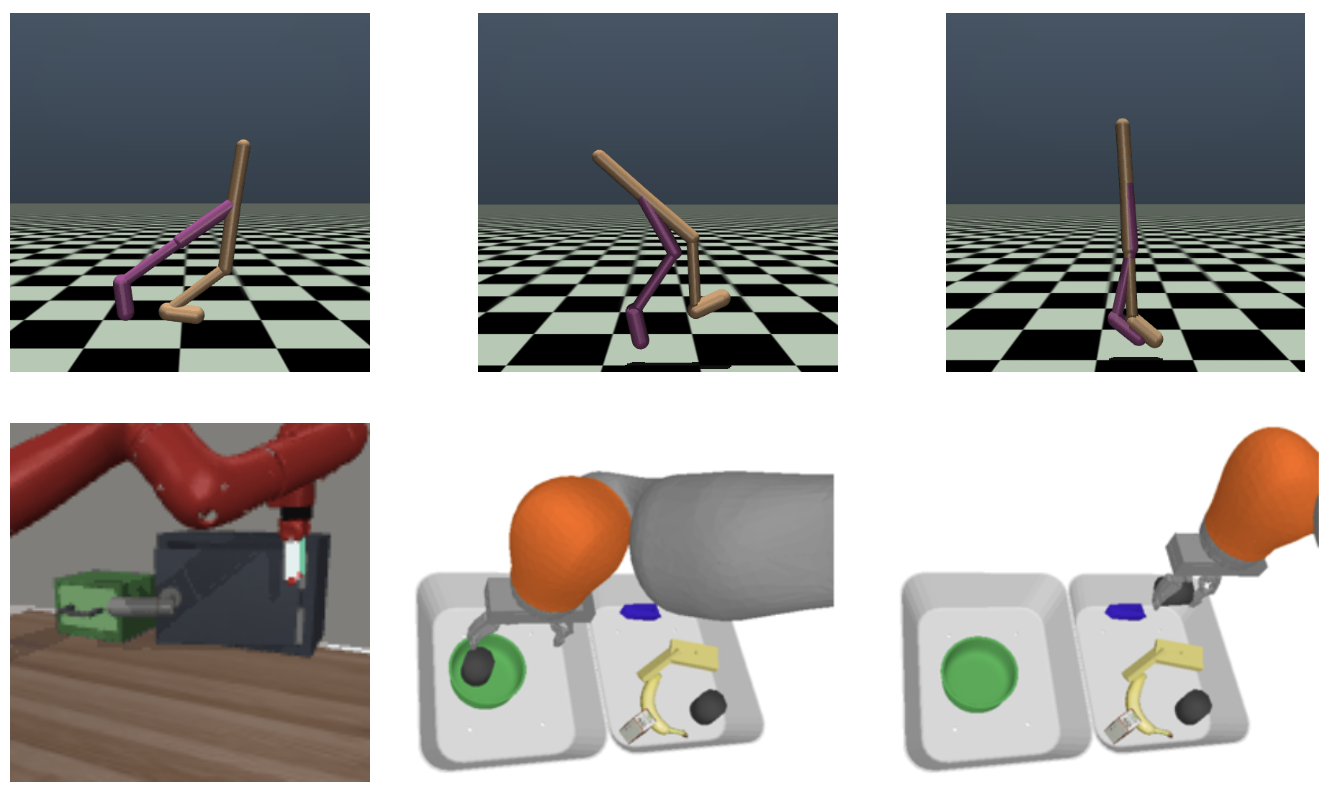
\includegraphics[width=0.65\textwidth]{chapters/cds/env.png}
    \vspace{-0.2cm}
    \caption{\footnotesize Visualization of our environments (from left to right): walker2d \texttt{run forward}, walker2d \texttt{run backward}, walker2d \texttt{jump},  Meta-World \texttt{door open/close} and \texttt{drawer open/close} and vision-based picking and placing tasks in \citep{kalashnikov2021mt}.}
    \label{fig:env}
    \vspace{-0.3cm}
\end{wrapfigure}

As shown in Table~\ref{tbl:gym}, \methodname\ achieves the best average success rate compared to prior methods. Note that without data sharing, the agent completely fails to solve most of the tasks due to the low quality of the medium replay datasets and the insufficient data for the expert datasets. \textbf{Sharing All} actually achieves second best results since in the sparse reward settings, data sharing can introduce more supervision signal and help training. \methodname\ further improves over \textbf{Sharing All}, suggesting that \methodname\ can not only prevent harmful data sharing, but also lead to more effective multi-task learning compared to \textbf{Sharing All} in scenarios where data sharing is imperative.

\textbf{Goal-conditioned AntMazes~\citep{fu2020d4rl}.} To answer question (4), we consider maze navigation tasks where the temporal ``stitching'' ability of an offline RL algorithm is crucial to obtain good performance. We create goal reaching tasks using the ant robot in the medium and hard mazes from \citet{fu2020d4rl}. The set of goals is a fixed discrete set of size 7 and 3 for large and medium mazes respectively. We modify the D4RL datasets for antmaze-*-play environments to construct two kinds of multi-task datasets: an ``undirected'' dataset, where data is equally divided between different tasks and the rewards are correspondingly relabeled, and a ``directed'' dataset, where a trajectory is associated with the goal closest to the final state of the trajectory. This means that the per-task data in the undirected setting may not be relevant to reaching the goal of interest. Thus, data-sharing is crucial to obtain good performance in this setting: methods that do not effectively perform data sharing and train on largely task-irrelevant data are expected to perform worse. Following \citep{fu2020d4rl}, a reward of +1 is given if the state is within a threshold radius of the goal. A rollout terminates as soon it reaches the goal of interest. 

Table~\ref{tbl:gym} presents the normalized score proposed in \citep{fu2020d4rl} on this setting, averaged across all goal-reaching tasks. Observe that \methodname\ performs better than \textbf{Sharing All} and drastically outperforms HIPI in all four settings. Perhaps surprisingly, \textbf{No Sharing} is a strong baseline, however, is significantly outperformed by \methodname\ in the harder setting with undirected data. Moreover, \methodname\ performs on-par or better in the undirected setting compared to the directed setting, indicating the effectiveness of \methodname\ in routing data in challenging settings. 

% \subsection{Results on image-based robotic manipulation tasks}
% \label{sec:mtopt_results}

\begin{table*}[t!]
\scriptsize
\centering
\vspace*{0.1cm}
\begin{tabular}{l|r|r|r|r|r}
\toprule
\textbf{Task Name} & \textbf{\methodname\ (ours)}& \textbf{HIPI}~\cite{eysenbach2020rewriting} & \textbf{Skill~\cite{kalashnikov2021mt}} & \textbf{Sharing All} & \textbf{No Sharing}\\ \midrule
\texttt{lift-banana} & \textbf{54.0\%} & 39.7\%  & 33.6\% & 45.6\% & 12.6\%\\
\texttt{lift-bottle} & \textbf{76.3\%} & 58.5\%  & 53.3\% & 42.8\% & 44.5\%\\
\texttt{lift-sausage} & \textbf{75.9\%}  & 65.6\%  & 62.5\% & 73.8\% & 55.2\%\\
\texttt{lift-milk}& \textbf{82.7\%} & 75.3\% & 62.8\% & 68.9\% & 58.9\%\\

\texttt{lift-food} & \textbf{70.3\%} & 64.6\% & 23.1\% & 64.9\% & 29.5\%\\
\texttt{lift-can} & \textbf{76.1\%} & 70.8\% & 37.6\%& 49.4\%& 41.8\%\\
\texttt{lift-carrot} & \textbf{80.4\%} & 70.1\%  & 69.4\% & 72.2\% & 63.1\%\\
\texttt{place-bowl} & 84.4\%  & 72.0\% & \textbf{84.5\%} & 64.7\% & 77.0\%\\
\texttt{place-plate} & \textbf{86.9\%}  & 82.2\% & 79.5\% & 75.1\% & 82.2\%\\
\texttt{place-divider-plate} & \textbf{89.4\%}  & 72.6\% & 81.0\% & 79.3\% & 84.7\%\\
%\midrule
\CC \textbf{average} & \CC \textbf{77.6\%}  & \CC 67.2\% & \CC 58.7\% & \CC 63.7\% & \CC 55.0\%\\
\bottomrule
\end{tabular}
\vspace{-0.2cm}
\caption{\footnotesize Results for multi-task vision-based robotic manipulation domains in \citep{kalashnikov2021mt}. We consider 7 tasks denoted as \texttt{lift-object} where the goal of each task is to lift a different object and 3 tasks denoted as \texttt{place-fixture} where the goal of each task is to place a lifted object onto different fixtures. The numbers are in success rates. \methodname\ outperforms both a skill-based data sharing strategy~\citep{kalashnikov2021mt} (\textbf{Skill}) and other data sharing methods on the average task success rate (highlighted in gray) and 9 out of 10 per-task success rate.
}
\label{tbl:mtopt}
\normalsize
\vspace{-0.6cm}
\end{table*}

\textbf{Image-based robotic manipulation domains.} To explore how \methodname\ scales to image-based manipulation tasks (question (5)), we introduce a simulation environment similar to the real setup presented in~\cite{kalashnikov2021mt}. The environment consists of 10 image-based manipulation tasks that involve different combinations of picking specific objects (banana, bottle, sausage, milk box, food box, can and carrot) and placing them in one of the three fixtures (bowl, plate and divider plate) (see example task images in Fig.~\ref{fig:env}).
We pick these tasks due to their resemblance to the setup introduced in~\cite{kalashnikov2021mt}, where the authors devised a skill-based data-sharing heuristic strategy (\textbf{Skill}) for data-sharing that significantly outperformed simple data-sharing alternatives. \textbf{Skill} manually defines two oracle skills ``picking'' and ``placing'' and shares all picking tasks share data with each other but does not share data with any of the placing tasks and vice-versa. Our goal is to compare \methodname\ to \textbf{Skill} among other baselines used in state-based experiments.
To create the offline dataset that is used for offline RL, we collect separate datasets for all the tasks individually by running online RL~\cite{kalashnikov2018scalable} until the task reaches medium-level performance (40\% for picking tasks and 80\% placing tasks). At that point, we merge the whole replay buffers from different tasks creating a final dataset of 100K RL episodes where each episode consists of 25 transitions. Since \methodname\ is applicable to any offline multi-task RL algorithm, we employ it as a separate data-sharing strategy in \citep{kalashnikov2021mt} while keeping the model architecture and all the other hyperparameters constant, which allows us to carefully evaluate the influence of data sharing in isolation. The results are reported in Table~\ref{tbl:mtopt}. \methodname\ outperforms both \textbf{Skill} and other approaches, indicating that \methodname\ is able to scale to high-dimensional observation inputs and removes the burden of sharing data based on manually designed skills.